\noindent How do we prune before training? In this chapter, we explore an principled way of pruning on a layer-level before training by imposing some necessary constraints on the architecture.
\begin{figure}[h]
\centering
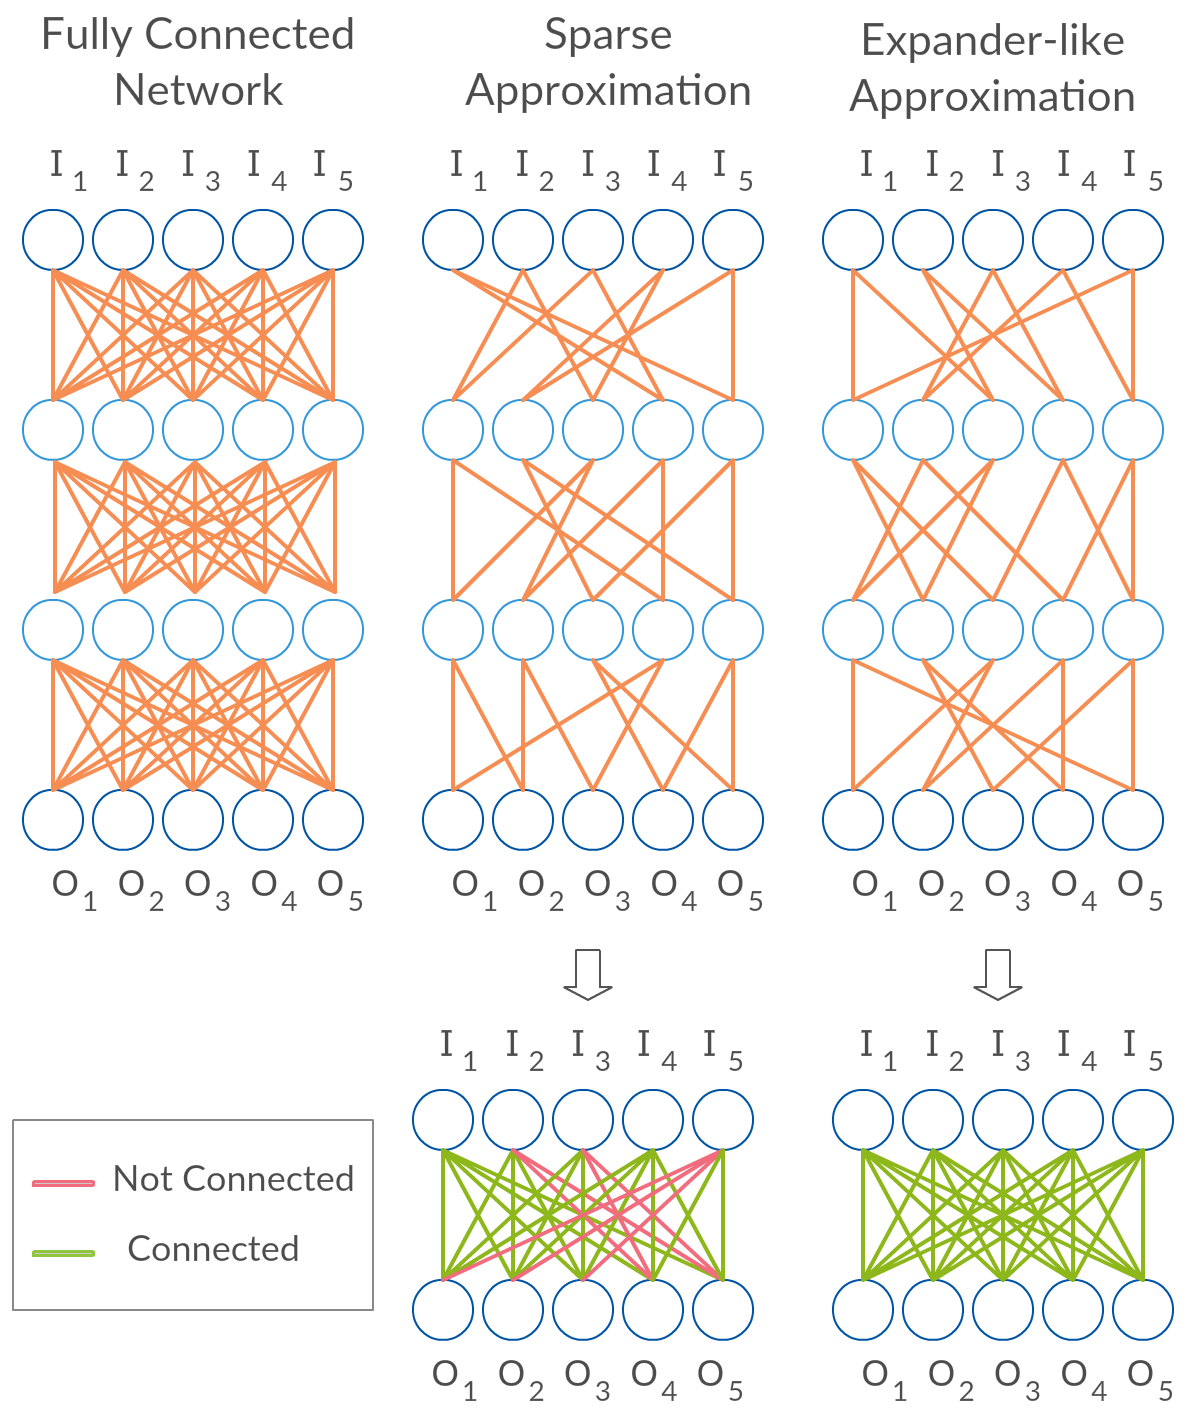
\includegraphics[width=0.4\textwidth]{figures/Expander2.png}
\caption{Popular sparse approximations are agnostic to the global information flow in a network, possibly creating disconnected components. In contrast, expander graph-based models produce sparse yet highly connected networks.}
\label{fig:intro}
\end{figure}

\section{Approach}\label{sec:approach}
\noindent Recent breakthroughs in CNN architectures like ResNet\cite{he2016deep} and DenseNet-BC\cite{huang2017densely} are ideas  based on increasing connectivity, which resulted in better performance trade-offs. These works suggest that connectivity is an important property for improving the performance of deep CNNs. In that vein, we investigate ways of preserving connectivity between neurons while significantly sparsifying the connections between them, shown in \ref{fig:intro}. Such networks are expected to preserve accuracy (due to connectivity) while being runtime efficient (due to the sparsity). We empirically demonstrate this in the later sections.

\subsection{Graphs and Deep CNNs}

\noindent We model the connections between neurons as graphs. This enables us to leverage well-studied concepts from Graph Theory like Expander Graphs. Now, we proceed to formally describe the connection between graphs and Deep CNNs.\\ 

\noindent {\bf Linear Layer defined by a Graph:} Given a bipartite graph $G$ with vertices $U, V$, the Linear layer defined by $G$, is a layer with $|U|$ input neurons, $|V|$ output neurons and each output neuron $v \in V$ is only connected to the neighbors given by $G$. Let the graph $G$ be sparse, having only $M$ edges. Then this layer has only $M$ parameters as compared to $|V|\times |U|$, which is the size of typical linear layers. \\
\noindent {\bf Convolutional Layer defined by a Graph:} Let a Convolutional layer be defined as a bipartite graph $G$ with vertices $U,V$ and a window size of $c\times c$. This layer takes a 3D input with $|U|$ channels and produces a 3D output with $|V|$ channels. The output channel corresponding to a vertex $v \in V$ is computed only using the input channels corresponding to the neighbors of $v$. Let $G$ be sparse, having only $M$ edges. Hence the kernel of this convolutional layer has $M \times c \times c$ parameters as compared to $|V|\times |U| \times c \times c$, which is the number of parameters in a vanilla CNN layer.

\subsection{Sparse Random Graphs}

\noindent We want to constrain  our convolutional layers to form a sparse graph $G$. Without any prior knowledge of the data distribution, we take inspiration from randomized algorithms and propose choosing the neighbours of every output neuron/channel uniformly and independently at random from the set of all its input channels. It is known that a graph $G$ obtained in this way belongs to a well-studied category of graphs called Expander Graphs, known to be sparse but well connected. \\

\noindent {\bf Expander Graph:} A bipartite expander with degree $D$ and spectral gap $\gamma$, is a bipartite graph $G=(U,V,E)$ ($E$ is the set of edges,  $ E \subseteq U\times V$) in which: \\

\noindent {\bf1.) Sparsity:} Every vertex in $V$ has only $D$ neighbors in $U$. We  will be using constructions with $D << |U|$. Hence the number of edges is only $D \times |V|$ as compared to $|U| \times |V|$ in a dense graph.\\

\noindent  {\bf 2.) Spectral Gap:} The eigenvalue with  the second largest absolute value $\lambda$ of the adjacency matrix is bounded away from D (the largest eigenvalue). Formally $1-\lambda/D \geq \gamma.$\\

\noindent {\bf Random expanders:} A random bipartite expander of degree $D$ on the two vertex sets $U, V$, is a graph in which for every vertex $v \in V$, the $D$ neighbors are chosen independently and uniformly from $U$. It is a well-known result in graph theory that such graphs have a large spectral gap (\cite{salil2012pseudo}). Similar to random expanders, there exist several explicit expander constructions. More details about explicit expanders can be found in the supplementary section.
We now proceed to give constructions of deep networks that have connections defined by an expander graph.\\

\noindent {\bf Expander Linear Layer (X-Linear):} The Expander Linear (X-Linear) layer is a layer defined by a random bipartite expander $G$ with degree $D$. The expander graphs that we use have values of $D << |U|$, while having an expansion factor of $K \approx D$, which ensures that the layer still has good expressive power.\\

\noindent {\bf Expander Convolutional Layer (X-Conv):} The Expander Convolutional (X-Conv) layer is a convolutional layer defined by a random bipartite expander graph $G$ with degree $D$, where $D << |U|$.\\ 

\noindent {\bf Deep Expander Networks (X-Nets):} Given expander graphs 
$$G_1 = (V_0,V_1,E_1), G_2 = (V_1,V_2,E_2), \cdots, G_t = (V_{t-1},V_t,E_t)$$, we define the Deep Expander Convolutional Network (Convolutional X-Net or simply X-Net) as a $t$ layer deep network in which the convolutional layers are replaced by X-Conv layers and linear layers are replaced by X-Linear layers defined by the corresponding graphs.

\begin{figure*}[t]
\centering
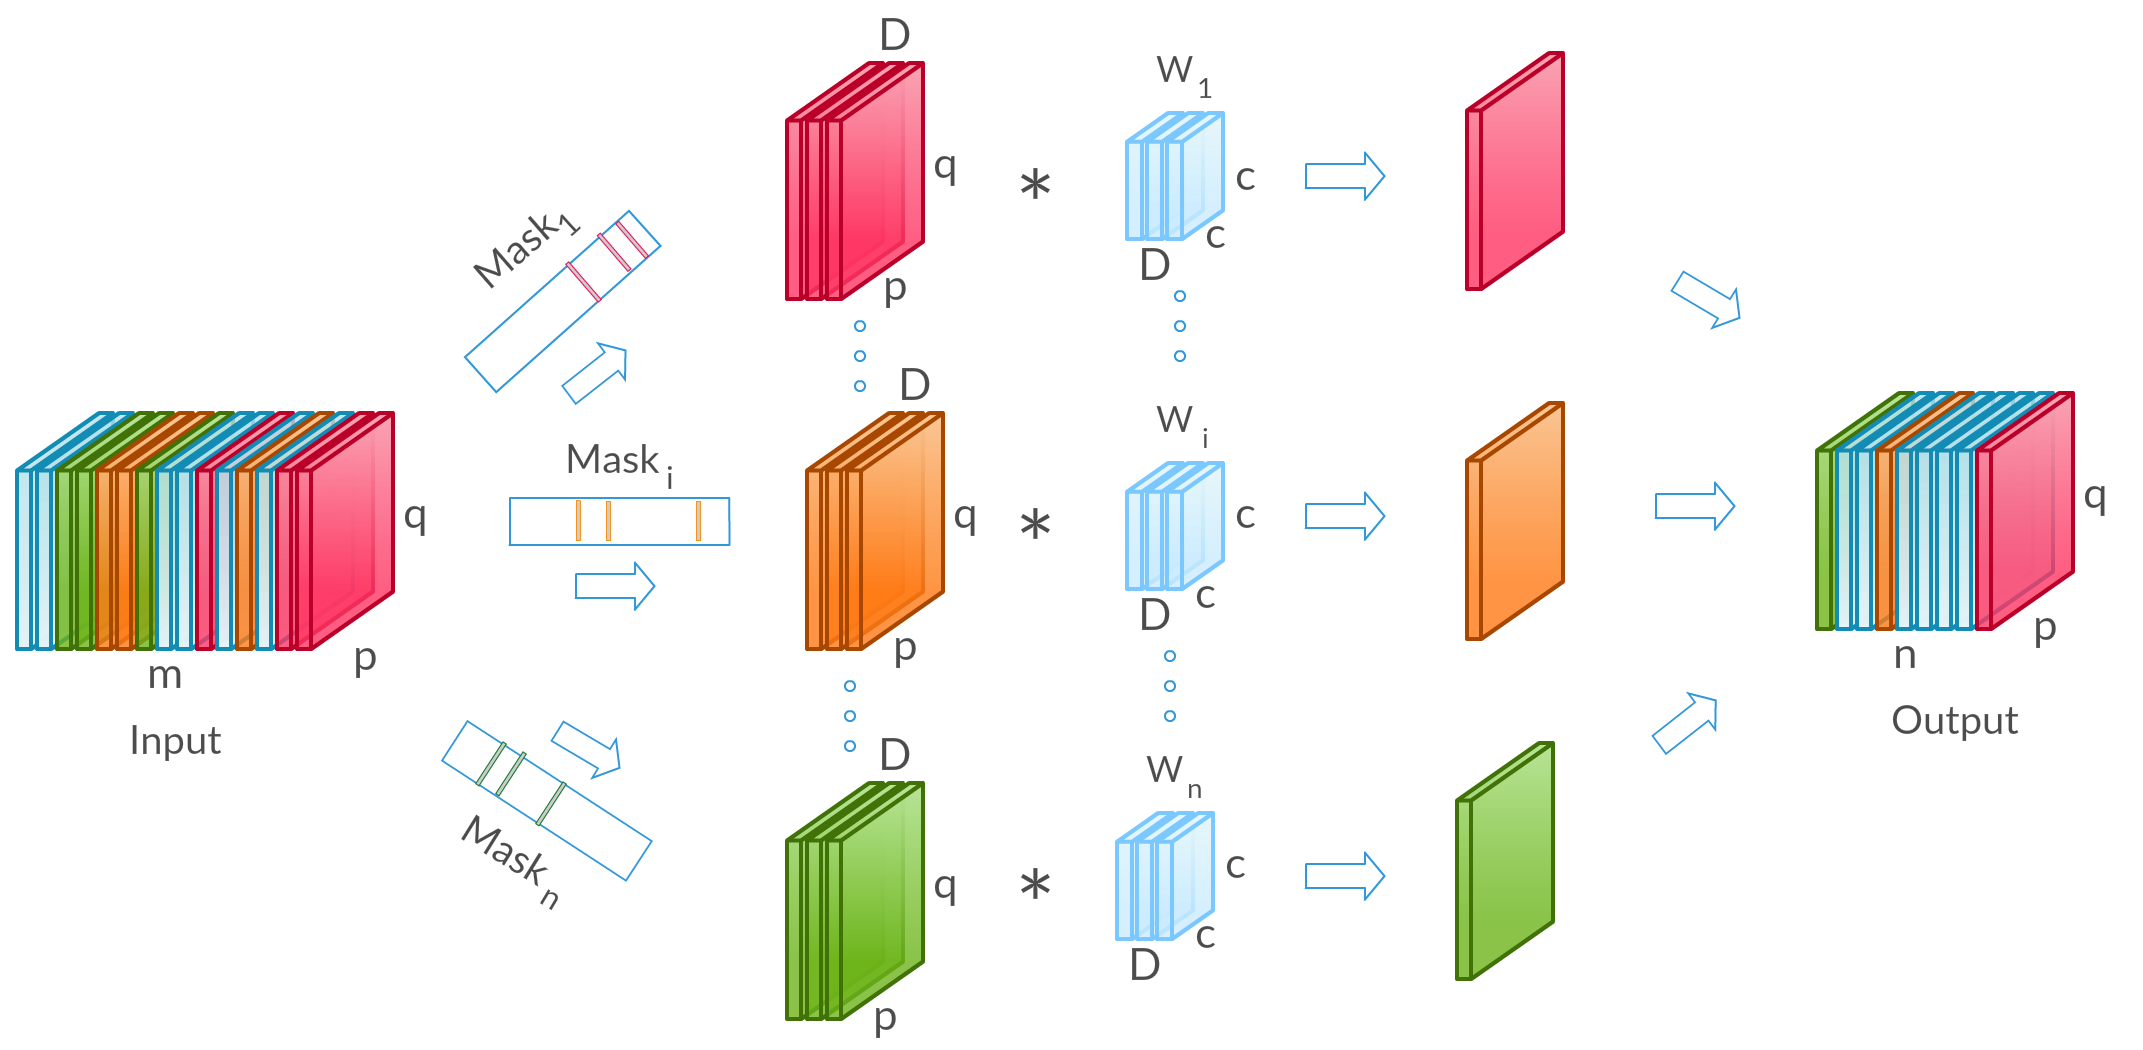
\includegraphics[width=1.0\textwidth]{figures/Expander.png}

\caption{The proposed fast convolution algorithm for X-Conv layer. We represent all the non-zero filters in the weight matrix of the X-Conv layer as a compressed dense matrix of $D$ channels. The algorithm starts by selecting $D$ channels from input (with replacement) using a mask created while initializing the model. The output is computed by convolving these selected channels with the compressed weight matrices.}
\label{fig:efficientmatrix}

\end{figure*}

\subsection{Measures of Connectivity}

\noindent In this subsection, we describe some connectivity properties of Expander graphs (see \cite{salil2012pseudo}, for the proofs). These will be used to prove the properties of sensitivity and mixing of random walks in X-Nets.\\

\noindent {\bf Expansion:} For every subset $S \subseteq V$ of size $\leq \alpha |V|$ ($\alpha \in (0,1)$ depends on the construction), let $N(S)$ be the set of neighbors. Then $|N(S)| \geq K |S|$ for $K\approx D$. That is, the neighbors of the vertices in $S$ are almost distinct. It is known that random expanders have expansion factor $K \approx D$ (see Theorem 4.4 in \cite{salil2012pseudo}).\\

\noindent {\bf Small Diameter:} The diameter of a graph is the length of the longest path among all shortest paths. If $G(U,V,E)$ is a $D$-regular expander with expansion factor $K > 1$ and diameter $d$, then  $d\leq O(\log n )$. This bound on the diameter implies that for any pair of vertices, there is a path of length $O(\log n)$ in the graph.\\

\noindent {\bf Mixing of Random Walks:} Random walks in the graph quickly converge to the uniform distribution over nodes of the graph. If we start from any vertex and keep moving to a random neighbor, in $O(\log n)$ steps the distribution will be close to uniform over the set of vertices.

\subsection{Sensitivity of X-Nets}

\noindent X-Nets have multiple layers, each of which have connections derived from an expander graph. We can guarantee that the output nodes in such a network are sensitive to all the input nodes.\\

\begin{theorem}[Sensitivity of X-Nets]\label{thm:conn}
Let $n$ be the number of input as well as output nodes in the network and $G_1,G_2,\cdots, G_t$ be $D$ regular bipartite expander graphs with $n$ nodes on both sides. Then  
every output neuron is sensitive to every input in a Deep X-Net defined by $G_i$'s with depth $t = O( \log n)$.

Proof: For every pair of input and output $(u,v)$, we show that there is a path in the X-Net. The proof is essentially related to the the fact that expander graphs have diameter $O(\log n)$. A detailed proof can be found in the Appendix B.
\end{theorem}

\noindent Next, we show a much stronger connectivity property known as mixing for the X-Nets. The theorem essentially says that the number of edges between subsets of input and output nodes is proportional to the product of their sizes. This result implies that the connectivity properties are uniform and rich across all nodes as well as subsets of nodes of the same size. Simply put, all nodes tend to have equally rich representational power.\\ 

\begin{theorem}[Mixing in X-Nets]
Let $n$ be the number of input as well as output nodes in the network and $G$ be $D$ regular bipartite expander graph with $n$ nodes on both sides. Let $S,T$ be subsets of input and output nodes in the X-Net layer defined by $G$. The number of edges between $S$ and $T$ is $\approx D|S||T|/n$.

Proof: A detailed proof is provided in the Appendix B.
\end{theorem}

\section{Efficient Algorithms}\label{sec:implementation}
 
\noindent In this section, we present efficient algorithms of X-Conv layers. Our algorithms achieve speedups and save memory in the training as well as the inference phase. This enables one to experiment with significantly wider and deeper networks given  memory and runtime constraints.
We exploit the structured sparsity of expander graphs to design fast algorithms.  We propose two methods of training X-Nets, both requiring substantially less memory and computational cost than their vanilla counterparts: \\1) Using Sparse Representations \\2) Expander-Specific Fast Algorithms.

\subsection{Using Sparse Representation}

\noindent The adjacency matrices of expander graphs are highly sparse for $D << n$. Hence, we can initialize a sparse matrix with non-zero entries corresponding to the edges of the expander graphs. Unlike most pruning techniques, the sparse connections are determined before training phase, and stay fixed. Dense-Sparse convolutions are easy to implement, and are supported by most deep learning libraries. CNN libraries like Cuda-convnet\cite{cudaconvnet} support such random sparse convolution algorithms.

 \begin{algorithm}[t]
 \textbf{Algorithm 1: } Fast Algorithm for Convolutions in X-Conv Layer\\
 \begin{algorithmic}[1]
 \State For every vertex $v \in \{1,\cdots, n\}$, let $N(v,i)$ denote the $i$th neighbor of $v$ ($i \in \{1,\cdots, D\}$).
 \State Let $K_v$ be the $c\times c \times D \times 1$ sized kernel associated with the $v$th output channel.
 \State Let $O_v[x,y]$ be the output value of the $v$th channel at the position $x,y$.
 \For{$v$= 1 to n}
     \State $O_v[x,y] = K_v * \textit{Mask}_{N(v,1),\cdots N(v,D)}(I)[x,y]$.
 \EndFor
 \end{algorithmic}
 \label{alg:cnnalgo}
 \end{algorithm}
 
 
\subsection{X-Net based Fast Dense Convolution}
\noindent Next, we present fast algorithms that exploit the sparsity of expander graphs.\\ %Moreover, our algorithm for X-Conv layers works for random expanders as well.

\noindent {\bf X-Conv:} In an X-Conv layer, every output channel is only sensitive to $out$ rom input channels. We propose to use a mask to select $D$ channels of the input, and then convolve with a $c \times c \times D \times 1$ kernel, obtaining a single channel per filter in the output. The mask is obtained by choosing D samples uniformly (without replacement) from the set $\{1,\cdots N\}$, where $N$ is the number of input channels. The mask value is $1$ for each of the selected $D$ channels and $0$ for others (see Algorithm \ref{alg:cnnalgo}). This is illustrated in Figure \ref{fig:efficientmatrix}. There has been recent work about fast CUDA implementations called Block-Sparse GPU Kernels\cite{blocksparse}, which can implement this algorithm efficiently.

\section{Experiments and Results}\label{sec:experiments}
\begin{figure}
\centering
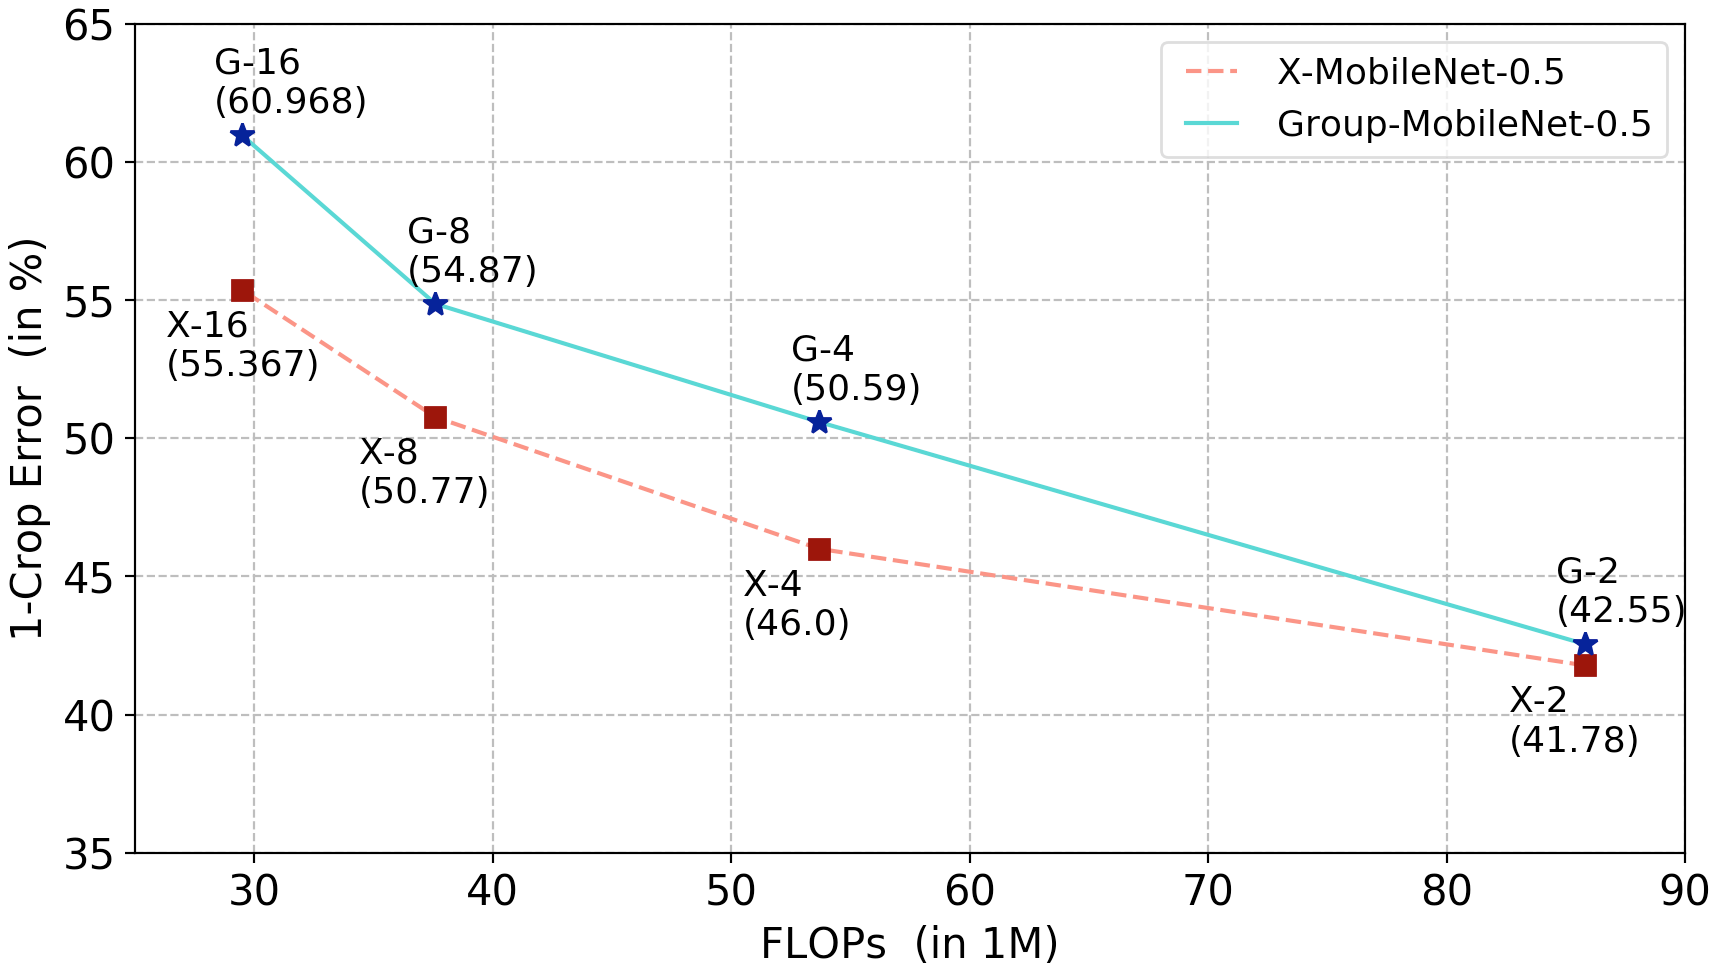
\includegraphics[width=0.55\textwidth]{figures/mobilenet.png}
\caption{Comparison between Grouped convolutions and X-Conv using MobileNet architecture trained on ImageNet. X-$d$ or G-$d$ represents the 1x1 conv layers are compressed by $d$ times using X-Conv or Groups. We observe X-MobileNets beat Group-MobileNet by 4\% in accuracy on increasing sparsity.}
\label{fig:mobilenet}
\end{figure}
\noindent In this section, we benchmark and empirically demonstrate the effectiveness of X-Nets on a variety of CNN architectures. Our code is available at: \url{https://github.com/DrImpossible/Deep-Expander-Networks}. 
\subsection{Comparison with Grouped Convolution}
\label{sec:group}


\noindent First, we compare our Expander Convolutions (X-Conv) against Grouped Convolutions (G-Conv). We choose G-Conv as it is a popular approach, on which a lot of concurrent works \cite{zhang2018shufflenet} have developed their ideas. G-Conv networks have the same sparsity as X-Conv networks but lack only the connectivity property. This will test whether increasing connectivity increases accuracy, i.e does a graph without good connectivity properties provides worse accuracy? We choose MobileNet as the base model for this experiment, since it is the state-of-the-art in efficient CNN architectures.\\
\begin{figure*}[t] 
\begin{tabular}{cc}
 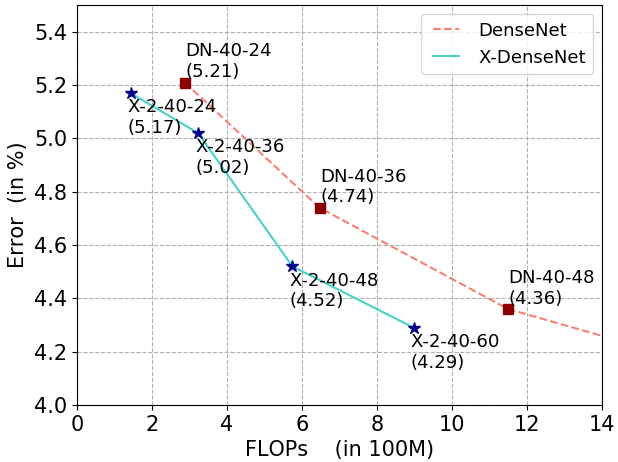
\includegraphics[width=0.5\textwidth]{figures/cifar10flops.png}  & 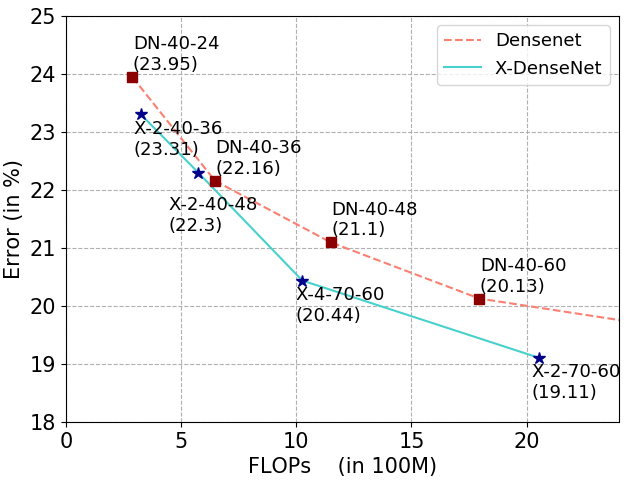
\includegraphics[width=0.5\textwidth] {figures/cifar100flops.png} \\
\\
(a) CIFAR10 & (b) CIFAR100 \\
\end{tabular}

\caption{We show the error as a function of \#FLOPs during test-time (below) for DenseNet-BC with X-DenseNet-BCs on CIFAR10 and CIFAR100 datasets. We observe X-DenseNet-BCs achieve better performance tradeoffs over DenseNet-BC models. For each datapoint, we mention the X-C-D-G notation (see Section \ref{sec:denres}) along with the accuracy.
}

\label{fig:cifar}
\end{figure*}
\noindent We compare X-Conv against grouped convolutions using MobileNet-0.5 on the ImageNet classification task. We replace the $1\times 1$ convolutional layers in MobileNet-0.5 with X-Conv layers forming X-MobileNet-0.5. Similarly, we replace them with G-Conv layers to form Group-MobileNet-0.5. Note that we perform this only in layers with most number of parameters (after the 8th layer as given in Table 1 of \cite{howard2017mobilenets}). We present our results in Figure \ref{fig:mobilenet}. The reference original MobileNet-0.5 has an error of 36.6\% with a cost of 150M FLOPs. Additional implementation details are given in the supplementary material.\\

\noindent We can observe that X-MobileNets beat Group-MobileNets by over 4\% in terms of accuracy when we increase sparsity. This also demonstrates that X-Conv can be used to further improve the efficiency of even the most efficient architectures like MobileNet.

\subsection{Comparison with Efficient CNN Architectures}
\label{sec:denres}

\noindent In this section, we test whether Expander Graphs can improve the performance trade-offs even in state-of-the-art architectures such as DenseNet-BCs \cite{huang2017densely} and ResNets\cite{he2016deep} on the ImageNet \cite{deng2009imagenet} dataset. We additionally train DenseNet-BCs on CIFAR-10 and CIFAR-100 \cite{krizhevsky2009learning} datasets to demonstrate the robustness of our approach across datasets.\\ 

\noindent Our X-ResNet-C-D is a $D$ layered ResNet that has every layer except the first and last replaced by an X-Conv layer that compresses connections between it and the previous layer by a factor of $C$. We compare across various models like ResNets-34,50,101. Similarly, our X-DenseNet-BC-C-D-G architecture has depth $D$, and growth rate $G$. We use DenseNet-BC-121-32,169-32,161-48,201-32 as base models. These networks have every layer except the first and last replaced by an X-Conv layer that compresses connections between it and the previous layer by a factor of $C$. More details are provided in the supplementary material.\\

\begin{figure}
\centering
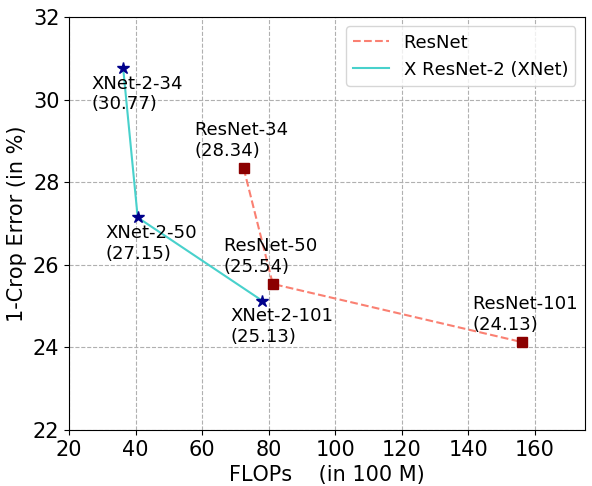
\includegraphics[width=0.55\textwidth]{figures/resnet.png}
\caption{We show the error as a function of \#FLOPs to compare between ResNet and X-ResNet on the ImageNet dataset. We observe X-ResNets achieve better performance tradeoffs over original ResNet models.}
\label{fig:resnet}
\end{figure}
   
 
\begin{table}
\centering
\begin{tabular}{|l|c|c|}
\hline
{\bf Model} & {\bf Accuracy}  & {\bf \#FLOPs}\\
\hline
ResNet &   & {\bf(in 100M)}\\
\hline
X-ResNet-2-34 & 69.23\%  & 35\\
X-ResNet-2-50 & {\bf 72.85\%}  & {\bf 40}\\
ResNet-34 & 71.66\%  & 70\\
X-ResNet-2-101 & {\bf 74.87\%}  & {\bf 80}\\
ResNet-50 & 74.46\%  & 80\\
ResNet-101 & 75.87\%  & 160\\
\hline
DenseNet-BC &  &   \\
\hline
X-DenseNet-BC-2-121 & 70.5\% & 28\\
X-DenseNet-BC-2-169 & 71.7\% & 33\\
X-DenseNet-BC-2-201 & 72.5\% & 43\\
X-DenseNet-BC-2-161 & {\bf 74.3\%} & {\bf 55}\\
DenseNet-BC-121 & 73.3\% & 55\\
DenseNet-BC-169 & 74.8\% & 65\\
DenseNet-BC-201 & 75.6\% & 85\\
DenseNet-BC-161 & 76.3\% & 110\\
\hline
\end{tabular}
      \caption{Results obtained by ResNet and DenseNet-BC models on ImageNet dataset, ordered by \#FLOPs. or each datapoint, we use the X-C-D-G notation (see Section \ref{sec:denres}) along with the accuracy.}
\label{tab:imagenet}
\end{table}
\subsection{Comparison with Pruning Techniques}
\label{sec:prun}

\noindent We plot the performance tradeoff of X-ResNets against ResNets in Figure \ref{fig:resnet} . We achieve significantly better performance tradeoffs compared to the original model. More specifically, we can reduce the \#FLOPs in ResNets by half while incurring only 1-1.5\% decrease in accuracy. Also, we can compare models with similar \#FLOPs or accuracy with the help of Table \ref{tab:imagenet}. We observe that  X-ResNet-2-50 has 43\% fewer FLOPs than ResNet-34, but achieves a 1\% improvement in accuracy against it. Similarly, X-DenseNet-BC-2-161 has similar \#FLOPs as DenseNet-BC-121, but achieves a 1\% improvement in accuracy. \\ 

\noindent To further prove the robustness of our approach on DenseNet-BC, we test the same on CIFAR10 and CIFAR100, and plot the tradeoff curve in Figure \ref{fig:cifar}.
We observe that we can achieve upto 33\% compression keeping accuracy constant on CIFAR-10 and CIFAR-100 datasets. \\

\noindent We compare our approach with methods which prune the weights during or after training. Our method can be thought of as constraining the weight matrices with a well studied sparse connectivity pattern even before the training starts. This results in fast training for the compact X-Conv models, while the trained pruning techniques face the following challenges: \\

\noindent 1) Slow initial training due to full dense model.\\
\noindent 2) Several additional phases of pruning and retraining.\\

\noindent Hence they achieve the compactness and runtime efficiency only in test time. Nevertheless we show similar sparsity can be achieved by our approach without explicitly pruning. We benchmark on VGG16 and AlexNet architectures since most previous results in the pruning literature have been reported on these architectures. In Table \ref{tab:cifar_fullcomp}, we compare two X-VGG-16 models against existing pruning techniques. We achieve comparable accuracies to the previous state-of-the-art model with 50\% fewer parameters and \#FLOPs. Similarly, in Table \ref{tab:imagenet_fullcomp} we compare X-AlexNet with trained pruning techniques on the Imagenet dataset. Despite having poor connectivity due to parameters being concentrated only in the last three fully connected layers, we achieve similar accuracy to AlexNet model using only 7.6M-9.7M parameters out of 61M, comparable to the state-of-the-art pruning techniques which have upto 3.4M-5.9M parameters. Additionally, it is possible to improve compression by applying pruning methods on our compact architectures, but pruning X-Nets is out of the scope of our current work.\\
\begin{table}[t]%{0.8\textwidth}
  \centering
\begin{tabular}{|l|c|c|}
\hline
{\bf Method} & {\sc { \bf Accuracy}} & {\bf \#Params} \\
 %&  &  & {\bf Speedup }?\\
\hline
Li et al. \cite{li2016pruning} & 93.4\%  & 5.4M \\
Liu et al. \cite{liu2017learning} &  93.8\% & 2.3M \\
\hline
X-VGG16-1 & 93.4\%  & 1.65M (9x) \\
X-VGG16-2 & 93.0\%  & 1.15M (13x) \\
\hline
VGG16-Orig &  94.0\% & 15.0M \\
\hline
\end{tabular}
\captionof{table}{Comparison with other methods on CIFAR-10 dataset using VGG16 as the base model. We significantly outperform popular compression techniques, achieving similar accuracies with upto 13x compression rate.}
\label{tab:cifar_fullcomp}
%\vspace{-0.6cm}
  \end{table}
  
\begin{table}[t]%{0.8\textwidth}
    \centering
\begin{tabular}{|l|c|c|}
\hline
{\bf Method} & {\bf Accuracy} & {\bf \#Params}\\ \hline
Network Pruning & & \\
\hline
Collins et al.\cite{collins2014memory} & 55.1\% & 15.2M \\
Zhou et al. \cite{zhou2016less} & 54.4\% & 14.1M \\
Han et al. \cite{han2015deep} &  57.2\% & 6.7M  \\
Han et al. \cite{han2015deep} & 57.2\% & 6.7M \\
 Srinivas et al. \cite{srinivas2017training} & 56.9\% & 5.9M \\
Guo et al. \cite{guo2016dynamic} & 56.9\% & 3.4M  \\
X-AlexNet-1 & 55.2\% & 7.6M  \\
X-AlexNet-2 & 56.2\% & 9.7M \\
\hline
AlexNet-Orig & 57.2\% & 61M \\
\hline
\end{tabular}
\captionof{table}{Comparison with other methods on ImageNet-2012 using AlexNet as the base model. We are able to achieve comparable accuracies using only 9.7M parameters.}
\label{tab:imagenet_fullcomp}
%\vspace{-0.6cm}
    \end{table}
  

\subsection{Stability of Models}
\noindent We give empirical evidence as well as a theoretical argument regarding the stability of our method. For the vanilla DNN training, the weights are randomly initialized, and randomized techniques like dropouts, augmentation are used. Hence there is some randomness present and is well accepted in DNN literature prior to our method. We repeat experiments on different datasets (Imagenet and CIFAR10) and architectures (VGG, DenseNet and MobileNet0.5) to empirically show that the accuracy of expander based models has variance similar to vanilla DNN training over multiple runs.\\

\noindent We repeated the experiments with independent sampling of random expanders on the VGG and DenseNet baselines on the CIFAR10 dataset. The results can be seen in Table~\ref{tab:cifar}. It is noted that the accuracy values changes only by less than $0.3$\% across runs and the standard deviation of expander method is also comparable to the vanilla DNN training.\\

\noindent We also repeated experiments of our main result, which is the comparison with grouped convolutions on ImageNet dataset. We rerun the experiment with MobileNet0.5 feature extractor twice with Groups and the expander method. As can be seen from Table~\ref{tab:imgnet}, the accuracy variations are comparable between the two models, and it is less than 1\%.\\

\begin{table}[!thb]
%\vspace{-2em}
\begin{minipage}{.5\linewidth}
\centering
\scalebox{0.9}{
\begin{tabular}{|l|c|c|c|c|}
\hline
{\bf Model} & {\bf Accuracy\%} & {\bf Max\%} & {\bf Min\%}\\
\hline
VGG & 93.96$\pm0.12$ & 94.17 & 93.67 \\
\hline
X-VGG-1 & 93.31$\pm0.18$ & 93.66 & 93.06 \\
X-VGG-2 & 92.91$\pm0.19$ & 93.26 & 92.69 \\
\hline
XDNetBC-40-24 & 94.41$\pm$0.19 & 94.63 & 94.18 \\
XDNetBC-40-36 & 94.98$\pm$0.14 & 95.21 & 94.84 \\
XDNetBC-40-48 & 95.49$\pm$0.15 & 95.65 & 95.28 \\
XDNetBC-40-60 & 95.75$\pm$0.07 & 95.81 & 95.68 \\

\hline
\end{tabular}}
%\vspace{0.5em}
\caption{The accuracies (mean $\pm$ stddev) of various models over 10 training runs on CIFAR-10 dataset.} \label{tab:cifar}
\end{minipage}%
\hfill
 \begin{minipage}{.45\linewidth}
 \centering
 \scalebox{0.9}{
\begin{tabular}{|c|c|c|}
\hline
{\bf MobileNet} & {\bf Mean} & {\bf Range}\\
{\bf Variant}  & {\bf Accuracy} & {\bf (Max-Min)}\\
\hline
Base & $63.39\%$ & $0.11\%$\\

\hline
G2 & $57.45~\%$ & $0.06~\%$\\
X2 & \bf{$58.22~\%$} & $ 0.14~\%$\\
\hline
G4 & $49.41~\%$ & $0.55~\%$\\
X4 & \bf{$54.00~\%$} & $0.53~\%$\\
\hline
G8 & $45.13~\%$ & $0.03~\%$\\
X8 & \bf{$49.23~\%$} & $0.60~\%$\\
\hline
G16 & $39.03~\%$ & $0.64~\%$\\
X16 & \bf{$44.63~\%$} & $0.18~\%$\\
\hline
\end{tabular}}
%\vspace{0.5em}\\
\caption{The mean accuracy and range of variation over  2 runs of MobileNet0.5 variants on ImageNet dataset.} \label{tab:imgnet}
\end{minipage}%
%\vspace{-3em}
\end{table}
\noindent A theoretical argument also concludes that choosing random graphs doesn't degrade stability. It is a well known result (See Theorem 4.4 in  \cite{salil2012pseudo}) in random graph theory, that graphs chosen randomly are well connected with overwhelmingly high probability (with only inverse exponentially small error, due to the Chernoff's Tail bounds) and satisfies the Expander properties. Hence the chance that for a specific run, the accuracy gets affected due to the selection of a particularly badly connected graph is insignificant.

\subsection{Training Wider and Deeper  networks}\label{sec:ultrawide}

\begin{figure*}[t]
\begin{tabular}{cc}

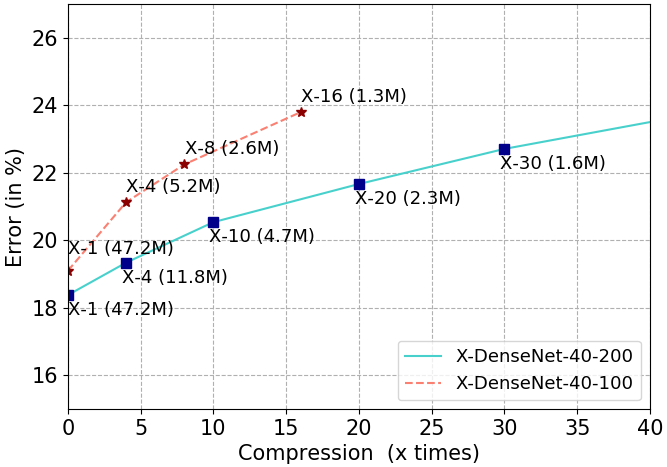
\includegraphics[width=0.5\textwidth]{figures/ultrawide.png}  & 
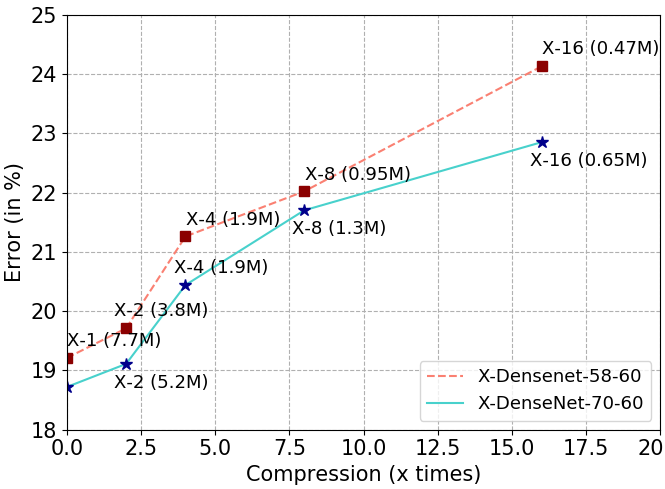
\includegraphics[width=0.5\textwidth] {figures/ultradeep.png}\\
(a) Effect of Width  & (b) Effect of Depth \\
\end{tabular}
\caption{We show the performance tradeoff obtained on training significantly wider and deeper networks on CIFAR-100 dataset. Every datapoint is X-$C$ specified along with the number of parameters, $C$ being the compression factor. We show that training wider or deeper networks along with more  compression using X-Nets achieve better accuracies with upto two-thirds of the total parameter and FLOPs on CIFAR-100 dataset. }
\label{fig:deepnet}
\end{figure*}

\noindent Since X-Nets involve constraining the weight matrices to sparse connectivity patterns before training, the fast algorithms can make it possible to utilize memory and runtime efficiently in training phase. This makes it possible to train significantly deeper and wider networks. Note the contrast with pruning techniques, where it is necessary to train the full, bulky model, inherently limiting the range of models that can be compressed.\\

\noindent Wide-DenseNets\footnote{https://github.com/liuzhuang13/DenseNet\#wide-densenet-for-better-timeaccuracy-and-memoryaccuracy-tradeoff} offered a better accuracy-memory-time trade-off. We increase the width and depth of these networks to train significantly wider and deeper networks. The aim is to study whether leveraging the effectiveness of X-Nets in this fashion can lead to better accuracies. \\
  
\noindent We widen and deepen the DenseNet-BC-40-60 architecture, increasing the growth rate from 60 to 100 and 200 respectively and compare the effect of increasing width on these new models. Similarly, we increase the depth from 40 to 58 and 70 to obtain deeper networks. We benchmark these approaches using CIFAR-100 dataset and present the results in Figure \ref{fig:deepnet}. \\

\noindent We have two interesting observations. First, the deeper X-DenseNet-BC-70-60 significantly outperforms X-DenseNet-BC-58-60 and wider X-DenseNet-40-200 outperforms X-DenseNet-BC-40-100 with fewer parameters for a wide range of $C$ values (Expander degree). \\

\noindent The second interesting observation is the decreasing slope of the curves. This  indicates that expander graph modeling seems to be effective on wider and deeper X-Nets i.e X-DenseNet-BC models suffer lesser penalty with increasing depth and width compression. This enables X-Nets to work at high compression rates of 30x, compressing DenseNet-BC-40-200 model from 19.9B FLOPs to 0.6B FLOPs with only $4.3\%$ drop in accuracy. We hope this preliminary investigation holds significant value in alleviating the constraint of GPU memory and resources.

\section{Summary}

\noindent We proposed a new network layer architecture for deep networks using expander graphs that give strong theoretical guarantees on connectivity. The resulting architecture (X-Net) is shown to be highly efficient in terms of both computational requirements and model size. In addition to being compact and computationally efficient, the connectivity properties of the network allow us to achieve significant improvements over the state-of-the-art architectures in performance on a parameter or run-time budget. In short, we show that the use of principled approaches that sparsify a model while maintaining global information flows can help in developing efficient deep networks. To the best of our knowledge, this is the first attempt at using theoretical results from graph theory in modeling connectivity to improve deep network architectures.